
%%
%% Template chap2.tex
%%

\chapter{Experiment 2: Learning with Thompson Sampling}
\label{cha:expt2}

\section{Experimental Protocol}
\label{sec:protocol2}

Studying Individual Heuristics
\begin{itemize}
	\item Split data into balanced training and test set. Use stratified shuffle split
	(similar to cross-validation) with 5 iterations
	\item Main classifier is logistic regression (one-vs-rest, L1-norm, $C=1$ for SDSS and $C=100$
	for VST ATLAS)
	\item Committee consists of 11 logistic classifiers
	\item Test 6 active learning heuristics with random sampling as benchmark
	\item Initial sample size is 50, train until we have 300 samples
	\item At each round, select a random sample of 300 and assign a score to each of them
\end{itemize}
Selection of Best Heuristic
\begin{itemize}
	\item Use Thompson Sampling to select best heuristic
	\item Still balanced split of training and test set, but now with 20 iterations of
	shuffle splits.
\end{itemize}

Two parts: balanced and unbalanced datasets. Both SDSS and VST ATLAS are not true
random samples of sky. E.g. in VST ATLAS, after corrected for bias, we should have [insert
table here]. Won't worry here since in practice, such survey never scan a random pathc
of sky anyway. Instead the surveys are results of other targeted projects.
The question that we're interested in, instead, is how well our algorithms can
deal with unbalanced data in general.


\section{Results and Discussion}
\label{sec:results2}
Margin appears to be the best performing heuristic in both SDSS and VST ATLAS.
To-do: add the maximum possible accuracy rate that can be achieved on plots

\subsection{Learning with the SDSS Dataset}




\begin{figure}[p]
	\centering
	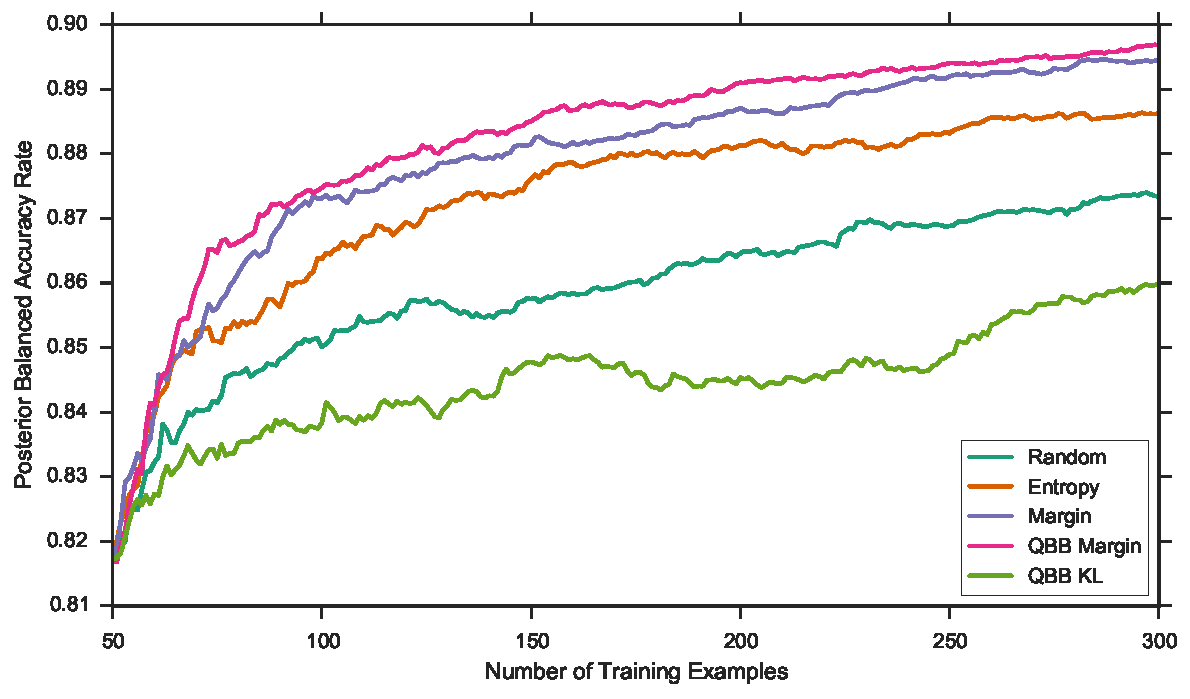
\includegraphics[width=\textwidth]{figures/5_active/sdss_bl_individuals}
	\caption[Learning with individual heuristics (SDSS, balanced, logistic)]{
		Learning with individual heuristics (SDSS, balanced, logistic)}
	\label{fig:sdss_bl_individuals}
\end{figure}

\begin{figure}[p]
	\centering
	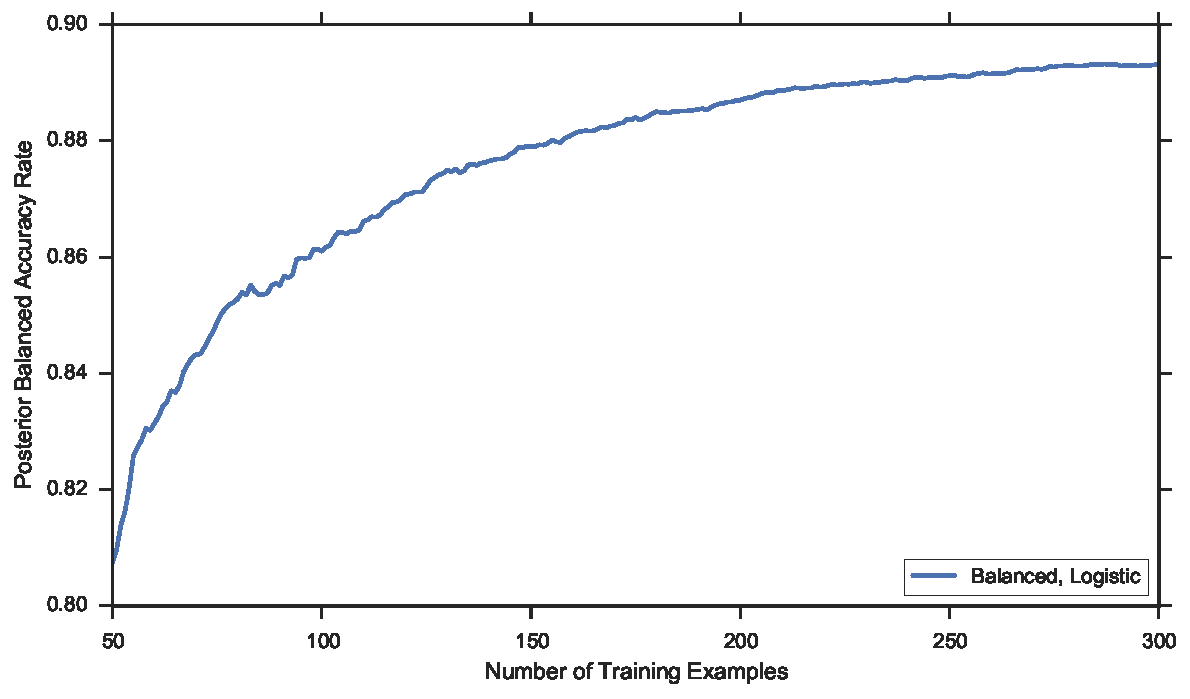
\includegraphics[width=\textwidth]{figures/5_thompson/sdss_bl_thompson}
	\caption[Learning with Thompson sampling (SDSS, balanced, logistic)]{
		Learning with Thompson sampling (SDSS, balanced, logistic)}
	\label{fig:sdss_bl_thompson}
\end{figure}

\begin{figure}[p]
	\centering
	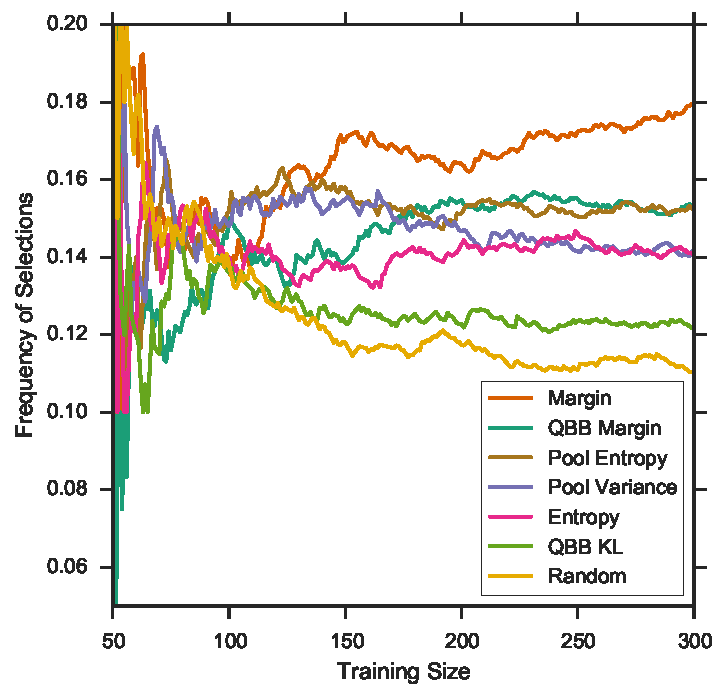
\includegraphics[width=\textwidth]{figures/5_thompson/sdss_bl_frequencies}
	\caption[Heuristic selection frequency (SDSS, balanced, logistic)]{
		Heuristic selection frequency (SDSS, balanced, logistic)}
	\label{fig:sdss_bl_frequencies}
\end{figure}

\begin{figure}[p]
	\centering
	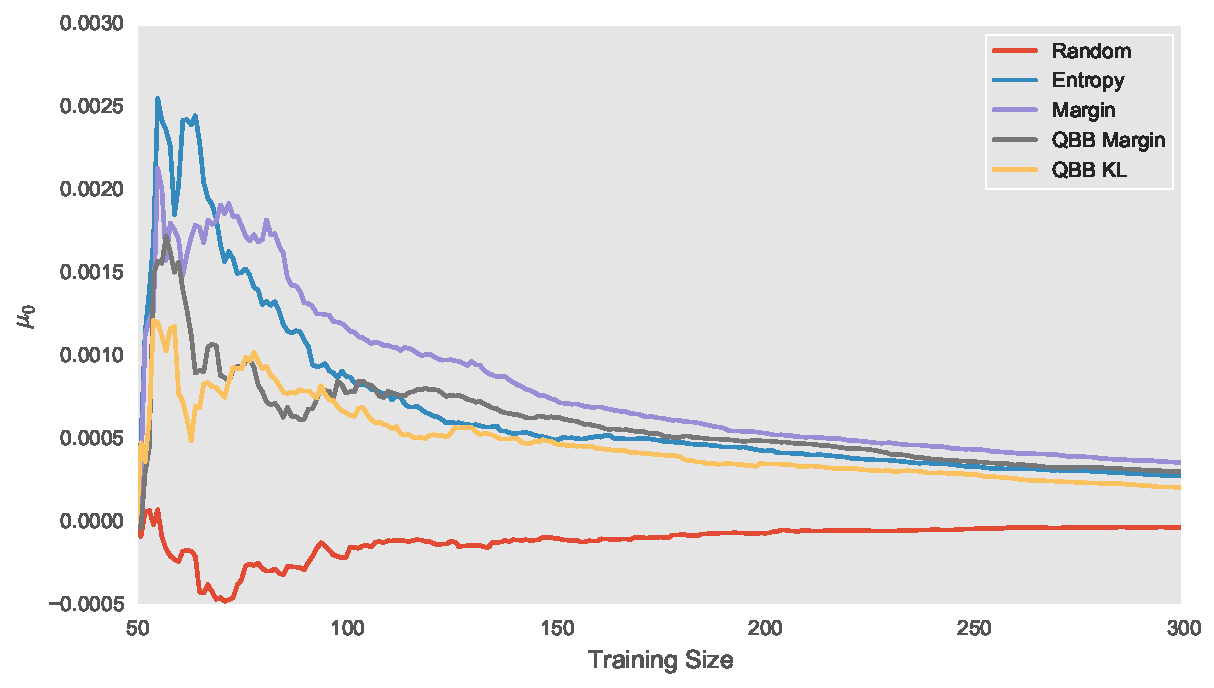
\includegraphics[width=\textwidth]{figures/5_thompson/sdss_bl_mus}
	\caption[Mean of the reward (SDSS, balanced, logistic)]{
		Mean of the reward (SDSS, balanced, logistic)}
	\label{fig:sdss_bl_mus}
\end{figure}

%--------------------------------------------------------------------------------------------------
\begin{figure}[p]
	\centering
	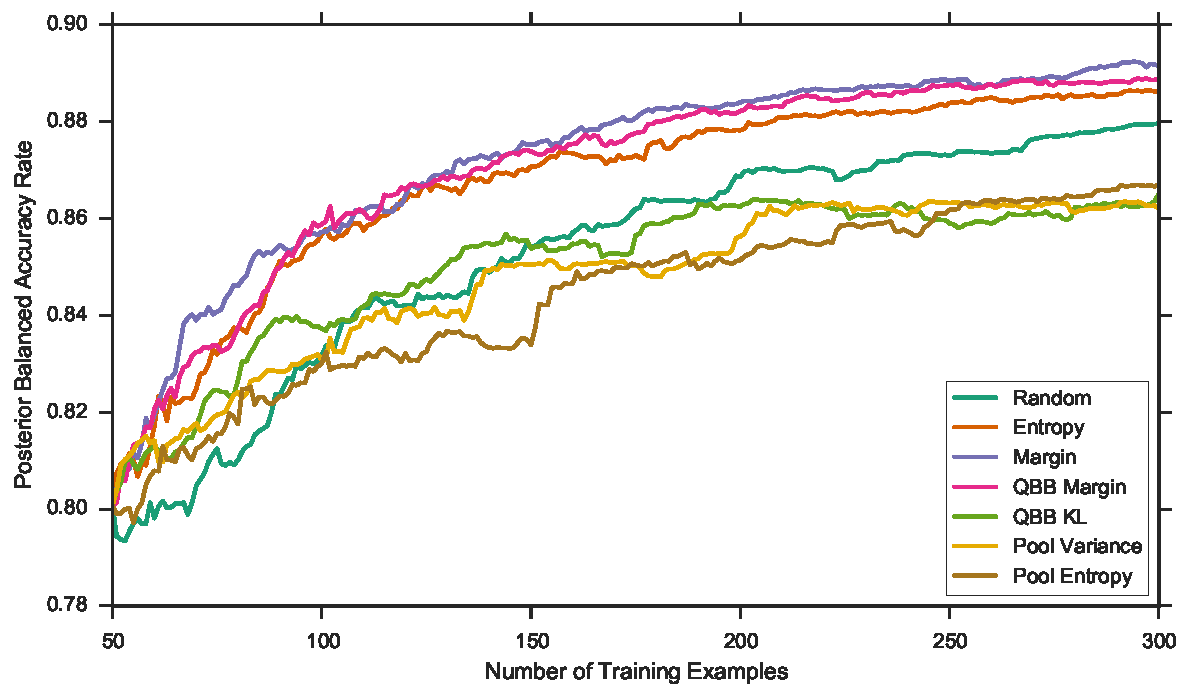
\includegraphics[width=\textwidth]{figures/5_active/sdss_br_individuals}
	\caption[Learning with individual heuristics (SDSS, balanced, SVM)]{
		Learning with individual heuristics (SDSS, balanced, SVM)}
	\label{fig:sdss_br_individuals}
\end{figure}

\begin{figure}[p]
	\centering
	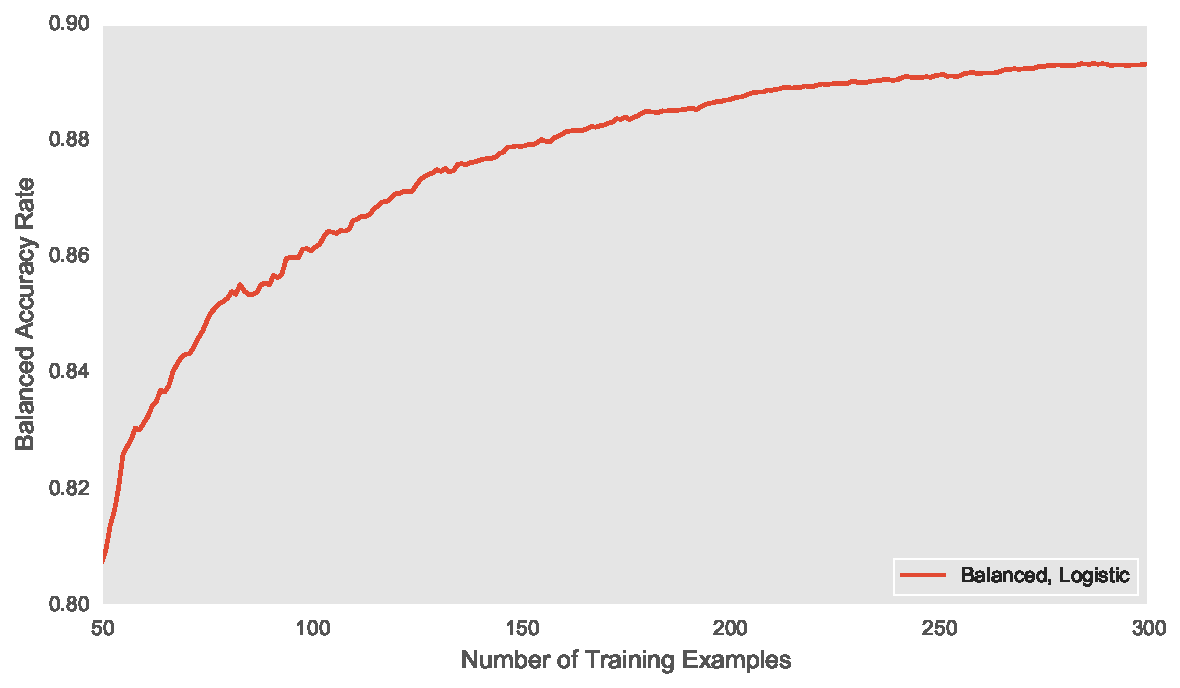
\includegraphics[width=\textwidth]{figures/5_thompson/sdss_br_thompson}
	\caption[Learning with Thompson sampling (SDSS, balanced, SVM)]{
		Learning with Thompson sampling (SDSS, balanced, SVM)}
	\label{fig:sdss_br_thompson}
\end{figure}

\begin{figure}[p]
	\centering
	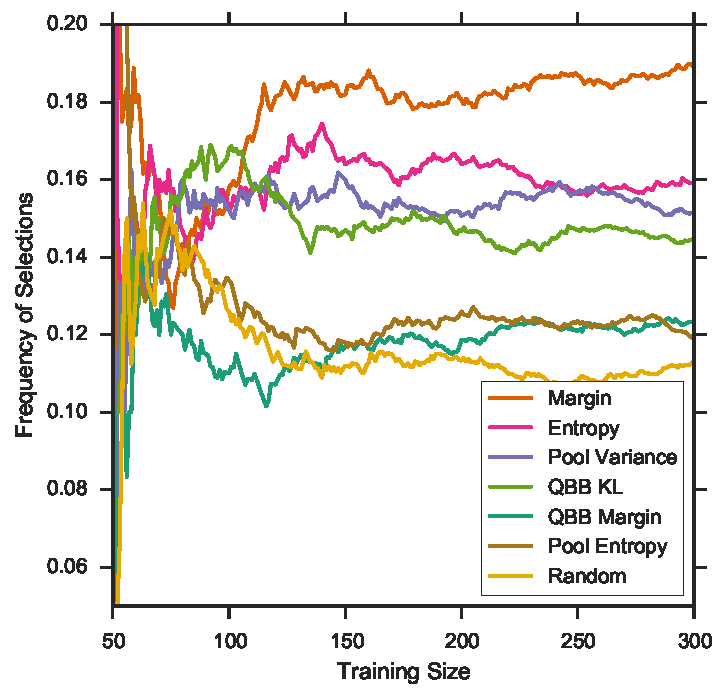
\includegraphics[width=\textwidth]{figures/5_thompson/sdss_br_frequencies}
	\caption[Heuristic selection frequency (SDSS, balanced, SVM)]{
		Heuristic selection frequency (SDSS, balanced, SVM)}
	\label{fig:sdss_br_frequencies}
\end{figure}

\begin{figure}[p]
	\centering
	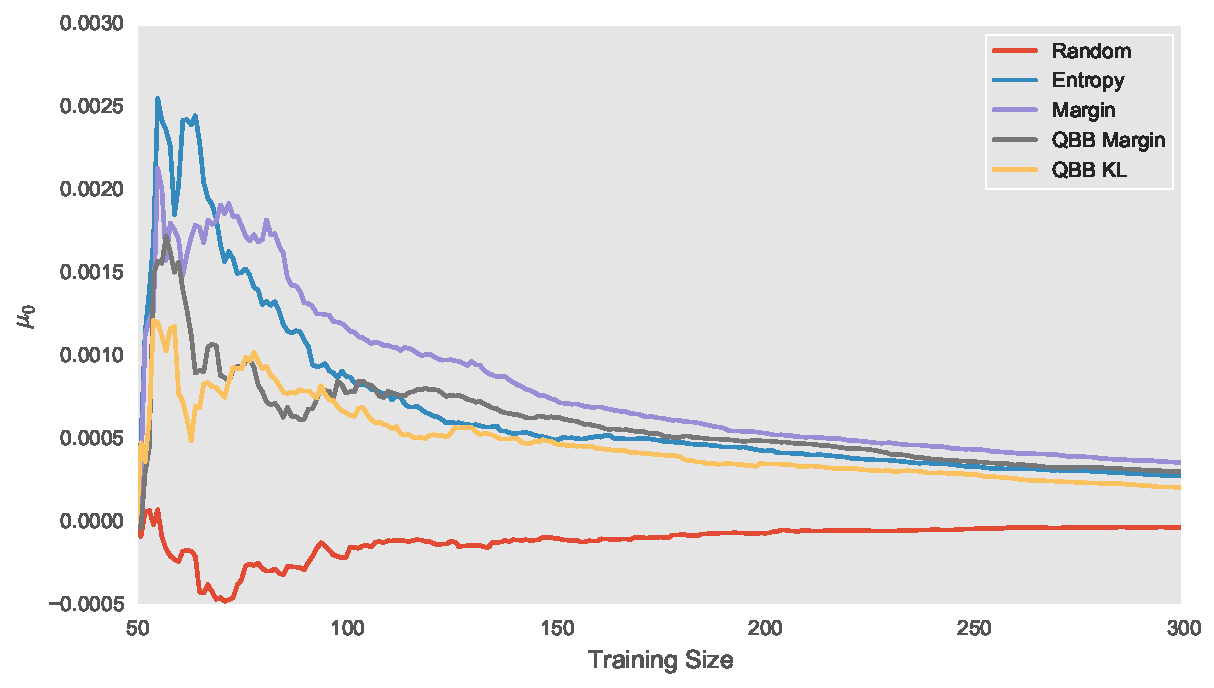
\includegraphics[width=\textwidth]{figures/5_thompson/sdss_br_mus}
	\caption[Mean of the reward (SDSS, balanced, SVM)]{
		Mean of the reward (SDSS, balanced, SVM)}
\end{figure}

%--------------------------------------------------------------------------------------------------
\begin{figure}[p]
	\centering
	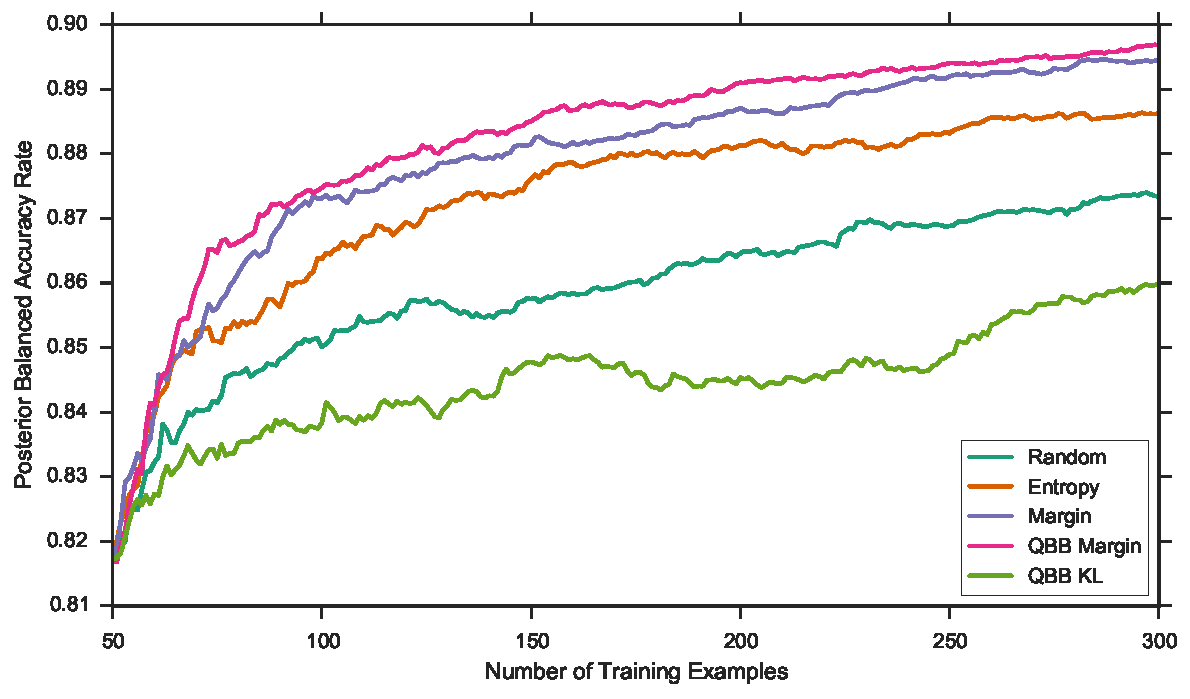
\includegraphics[width=\textwidth]{figures/5_active/sdss_ul_individuals}
	\caption[Learning with individual heuristics (SDSS, unbalanced, logistic)]{
		Learning with individual heuristics (SDSS, balanced, logistic)}
	\label{fig:sdss_ul_individuals}
\end{figure}

\begin{figure}[p]
	\centering
	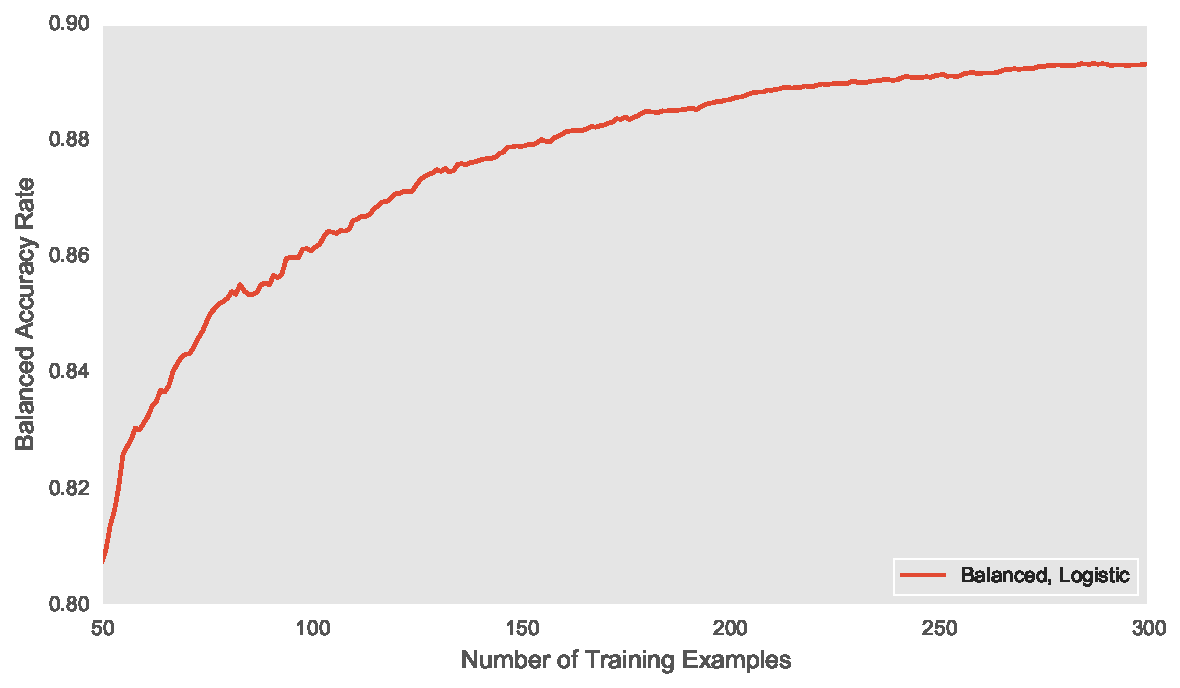
\includegraphics[width=\textwidth]{figures/5_thompson/sdss_ul_thompson}
	\caption[Learning with Thompson sampling (SDSS, unbalanced, logistic)]{
		Learning with Thompson sampling (SDSS, balanced, logistic)}
	\label{fig:sdss_ul_thompson}
\end{figure}

\begin{figure}[p]
	\centering
	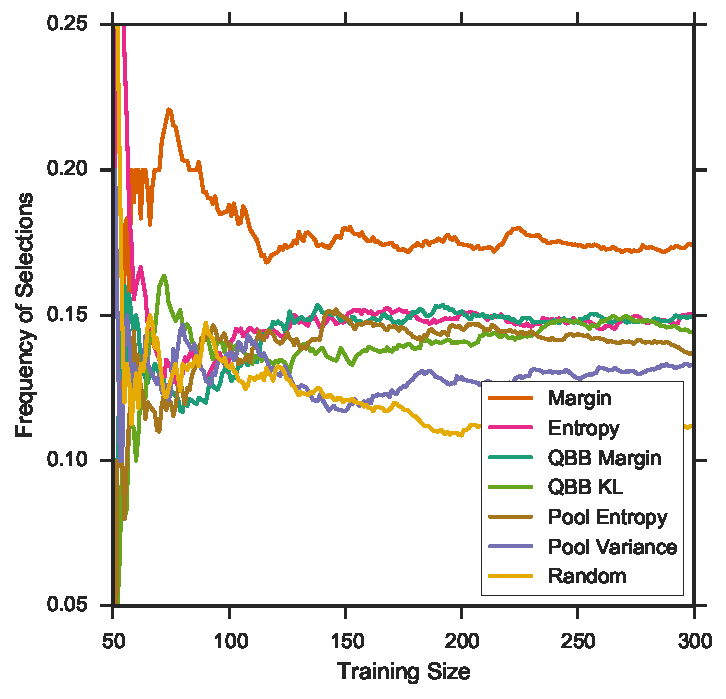
\includegraphics[width=\textwidth]{figures/5_thompson/sdss_ul_frequencies}
	\caption[Heuristic selection frequency (SDSS, unbalanced, logistic)]{
		Heuristic selection frequency (SDSS, balanced, logistic)}
	\label{fig:sdss_ul_frequencies}
\end{figure}

\begin{figure}[p]
	\centering
	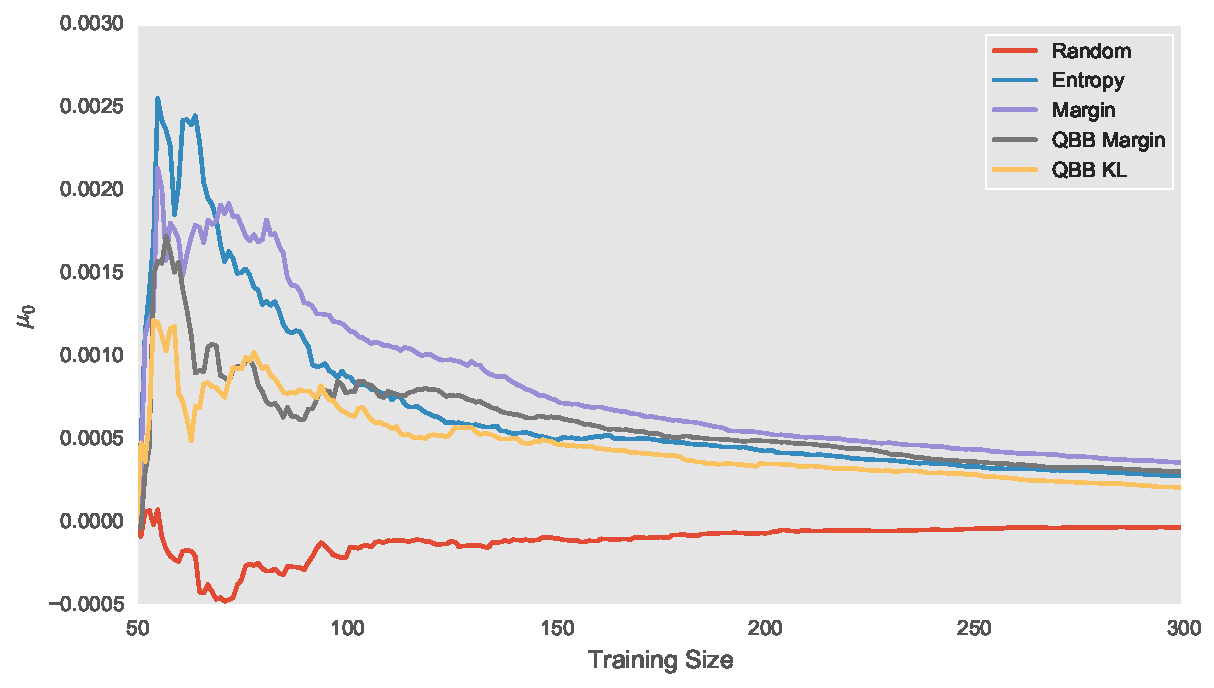
\includegraphics[width=\textwidth]{figures/5_thompson/sdss_ul_mus}
	\caption[Mean of the reward (SDSS, unbalanced, logistic)]{
		Mean of the reward (SDSS, balanced, logistic)}
\end{figure}

%--------------------------------------------------------------------------------------------------
\begin{figure}[p]
	\centering
	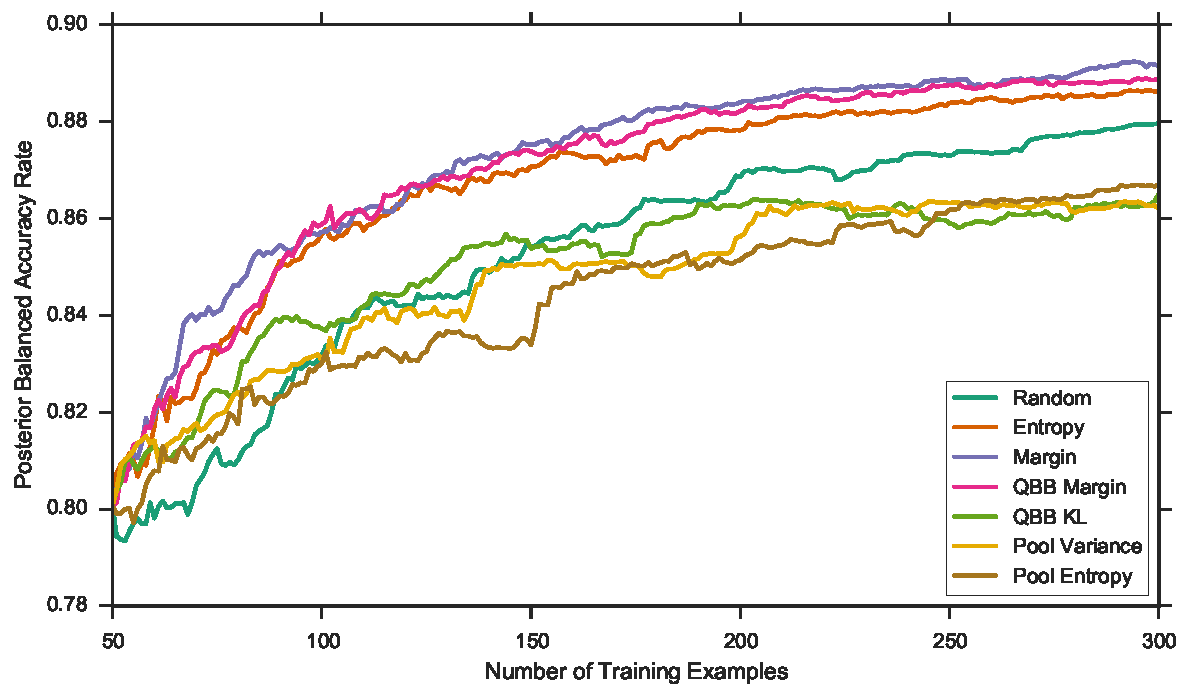
\includegraphics[width=\textwidth]{figures/5_active/sdss_ur_individuals}
	\caption[Learning with individual heuristics (SDSS, unbalanced, SVM)]{
		Learning with individual heuristics (SDSS, balanced, SVM)}
	\label{fig:sdss_ur_individuals}
\end{figure}

\begin{figure}[p]
	\centering
	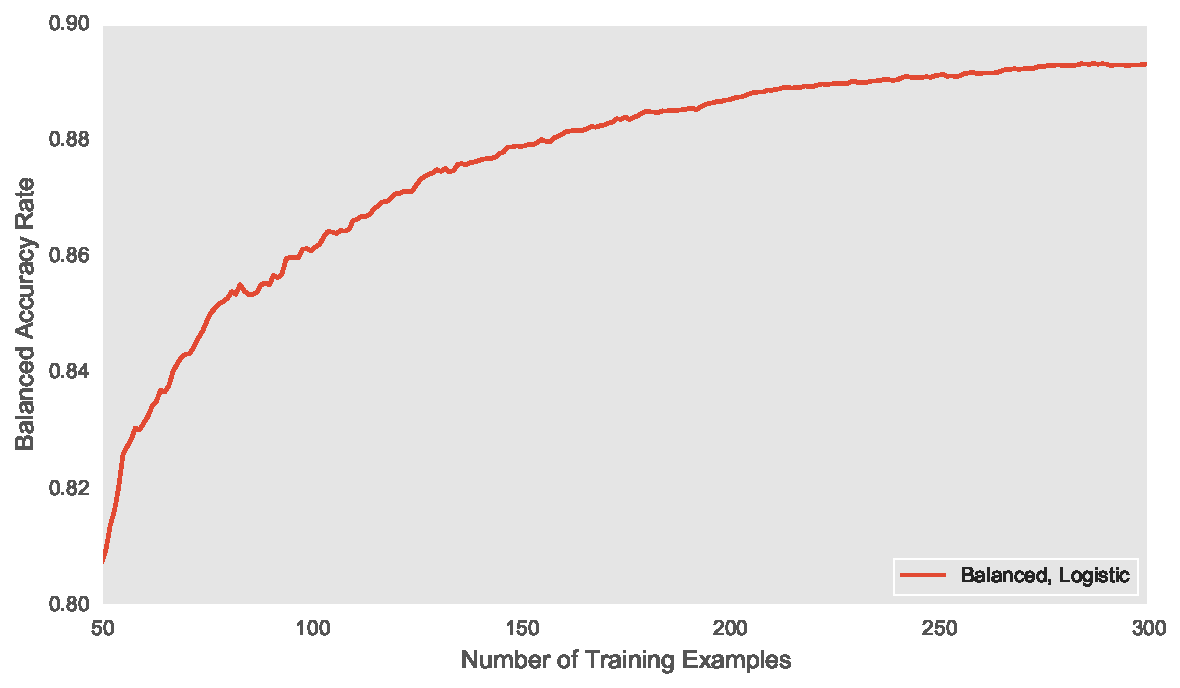
\includegraphics[width=\textwidth]{figures/5_thompson/sdss_ur_thompson}
	\caption[Learning with Thompson sampling (SDSS, unbalanced, SVM)]{
		Learning with Thompson sampling (SDSS, balanced, SVM)}
	\label{fig:sdss_ur_thompson}
\end{figure}

\begin{figure}[p]
	\centering
	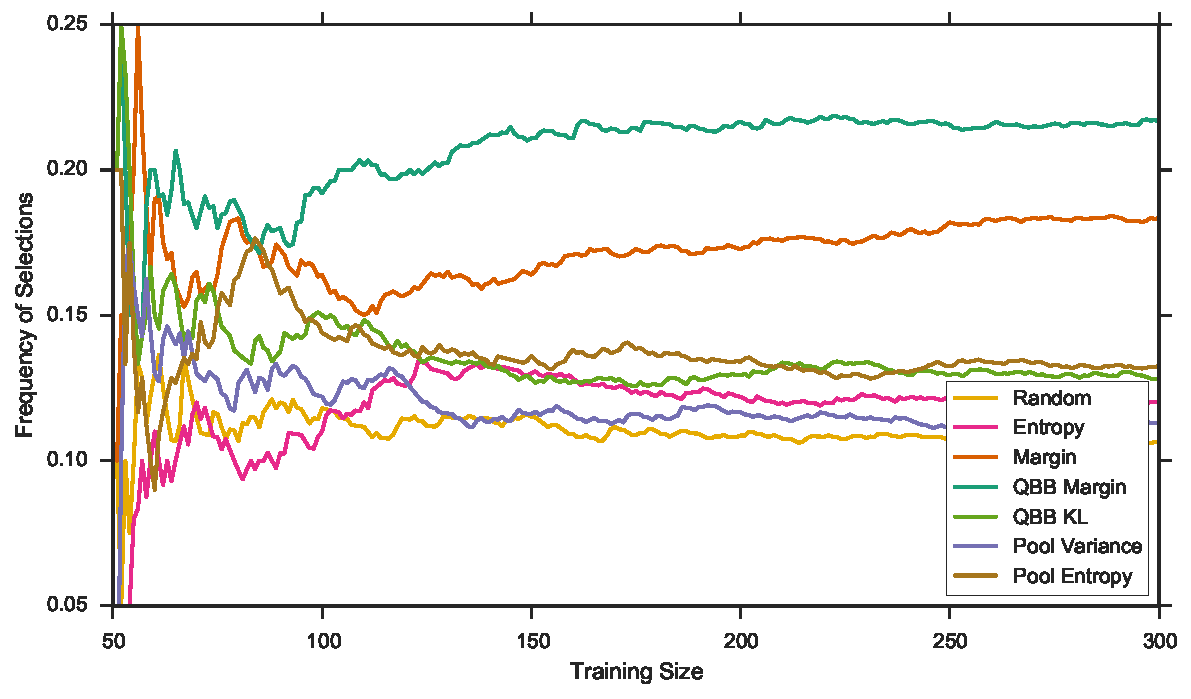
\includegraphics[width=\textwidth]{figures/5_thompson/sdss_ur_frequencies}
	\caption[Heuristic selection frequency (SDSS, unbalanced, SVM)]{
		Heuristic selection frequency (SDSS, balanced, SVM)}
	\label{fig:sdss_ur_frequencies}
\end{figure}

\begin{figure}[p]
	\centering
	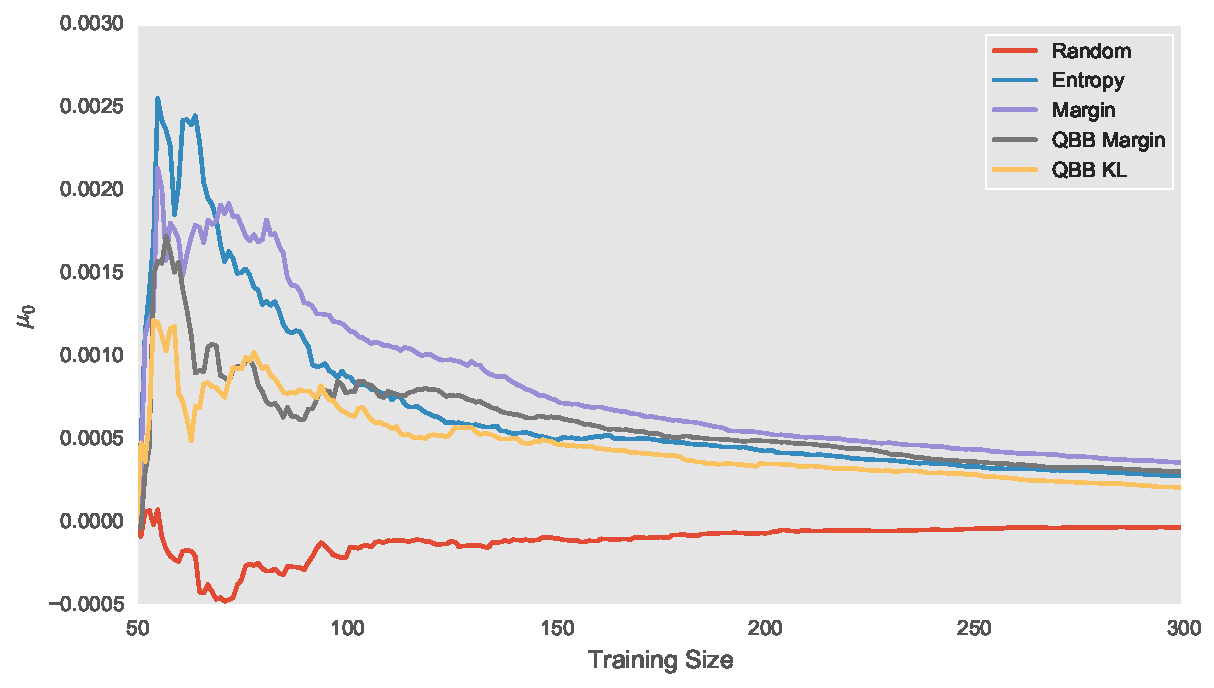
\includegraphics[width=\textwidth]{figures/5_thompson/sdss_ur_mus}
	\caption[Mean of the reward (SDSS, unbalanced, SVM)]{
		Mean of the reward (SDSS, balanced, SVM)}
\end{figure}



\clearpage
% % % % % % % % % % % % % % % % % % % % % % % % % % % % % % % % % % % % % % % % % % % % % % % % % %
\subsection{Learning with the VST ATLAS Dataset}

\begin{figure}[p]
	\centering
	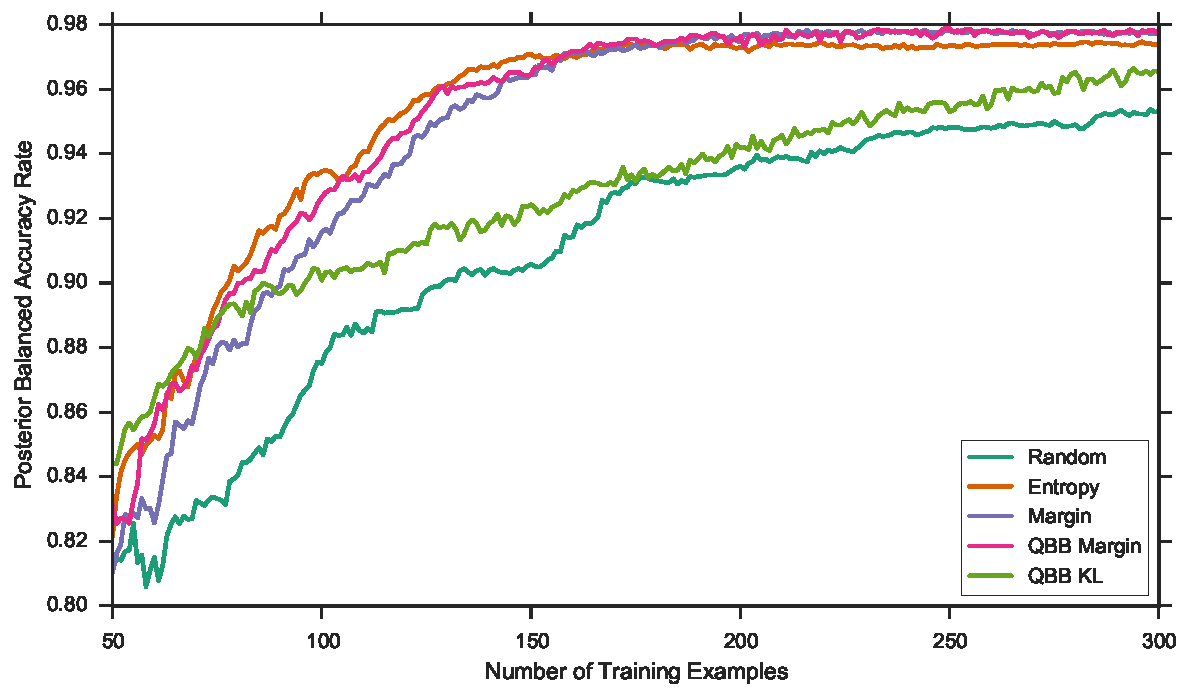
\includegraphics[width=\textwidth]{figures/5_active/vstatlas_bl_individuals}
	\caption[Learning with individual heuristics (VST ATLAS, balanced, logistic)]{
		Learning with individual heuristics (VST ATLAS, balanced, logistic)}
	\label{fig:vstatlas_bl_individuals}
\end{figure}

\begin{figure}[p]
	\centering
	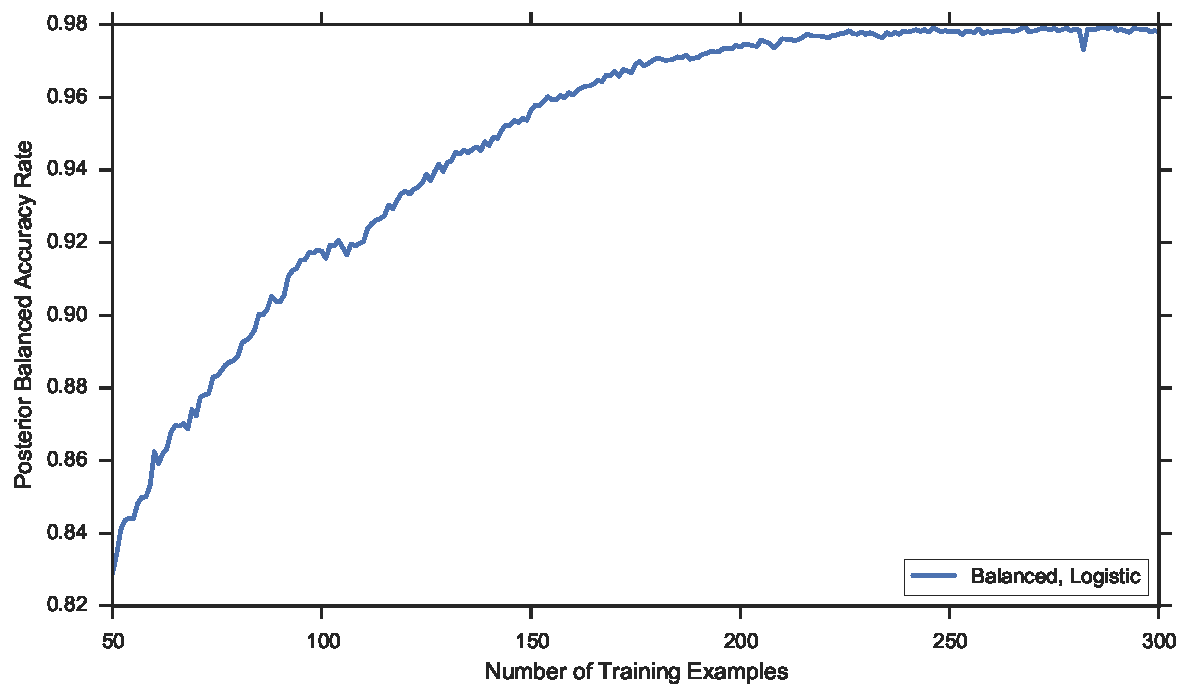
\includegraphics[width=\textwidth]{figures/5_thompson/vstatlas_bl_thompson}
	\caption[Learning with Thompson sampling (VST ATLAS, balanced, logistic)]{
		Learning with Thompson sampling (VST ATLAS, balanced, logistic)}
	\label{fig:vstatlas_bl_thompson}
\end{figure}

\begin{figure}[p]
	\centering
	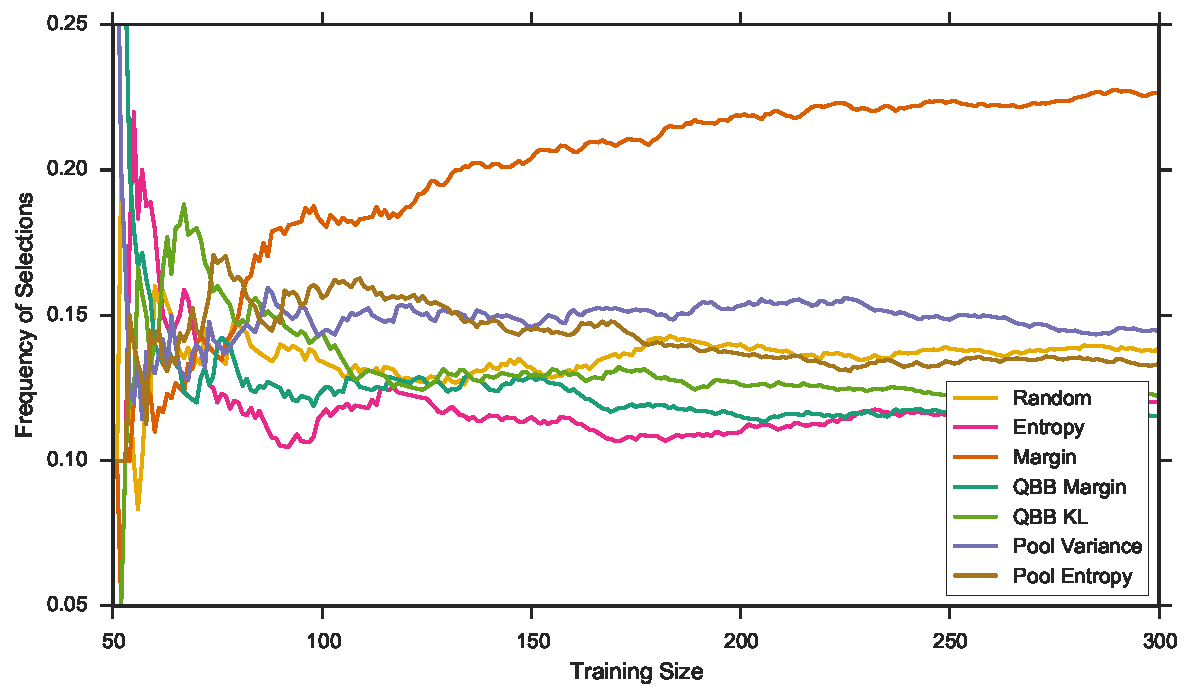
\includegraphics[width=\textwidth]{figures/5_thompson/vstatlas_bl_frequencies}
	\caption[Heuristic selection frequency (VST ATLAS, balanced, logistic)]{
		Heuristic selection frequency (VST ATLAS, balanced, logistic)}
	\label{fig:vstatlas_bl_frequencies}
\end{figure}

\begin{figure}[p]
	\centering
	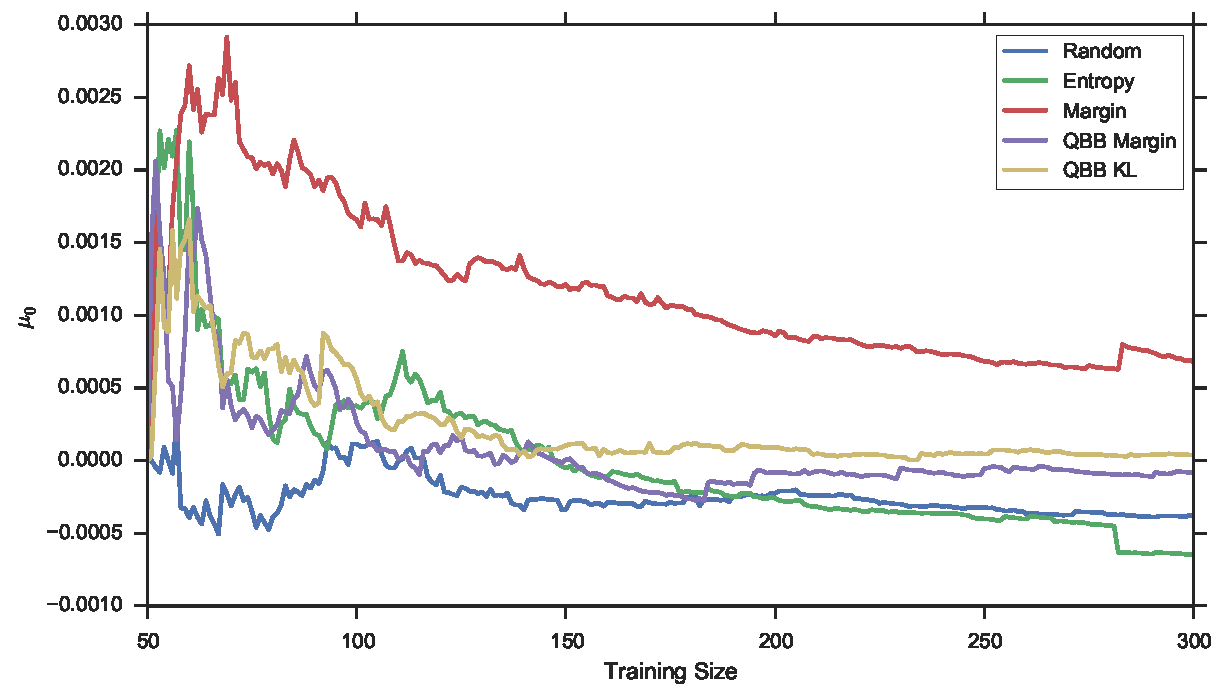
\includegraphics[width=\textwidth]{figures/5_thompson/vstatlas_bl_mus}
	\caption[Mean of the reward (VST ATLAS, balanced, logistic)]{
		Mean of the reward (VST ATLAS, balanced, logistic)}
	\label{fig:vstatlas_bl_mus}
\end{figure}

%--------------------------------------------------------------------------------------------------
\begin{figure}[p]
	\centering
	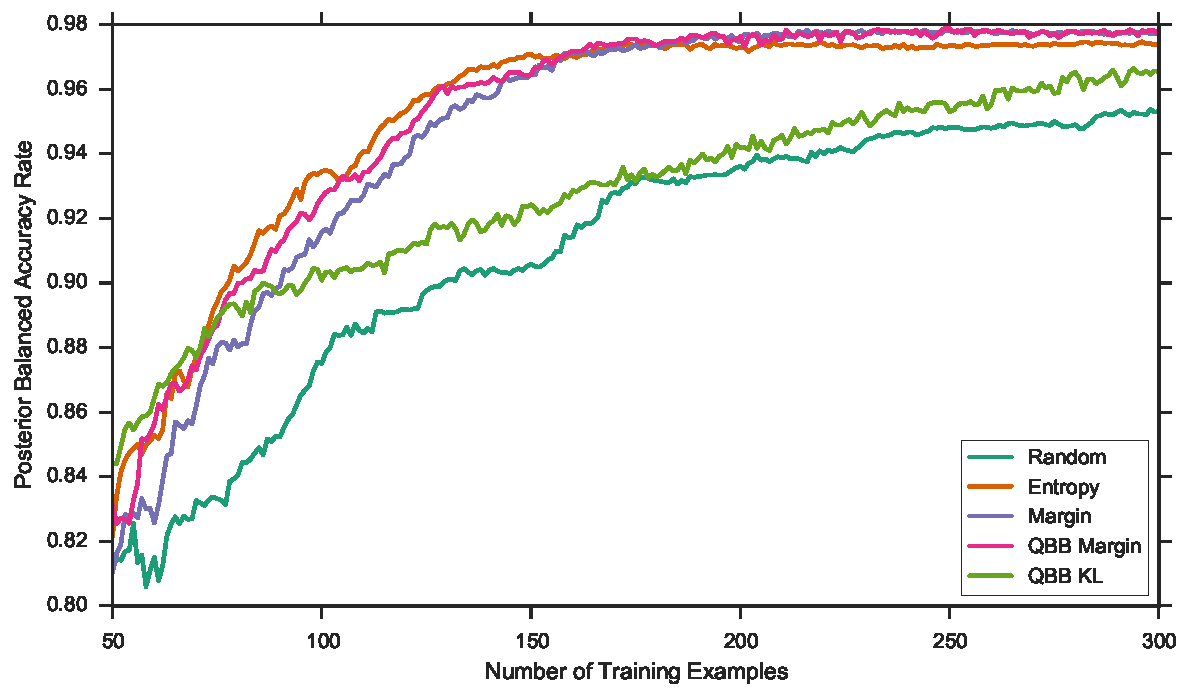
\includegraphics[width=\textwidth]{figures/5_active/vstatlas_br_individuals}
	\caption[Learning with individual heuristics (VST ATLAS, balanced, SVM)]{
		Learning with individual heuristics (VST ATLAS, balanced, SVM)}
	\label{fig:vstatlas_br_individuals}
\end{figure}

\begin{figure}[p]
	\centering
	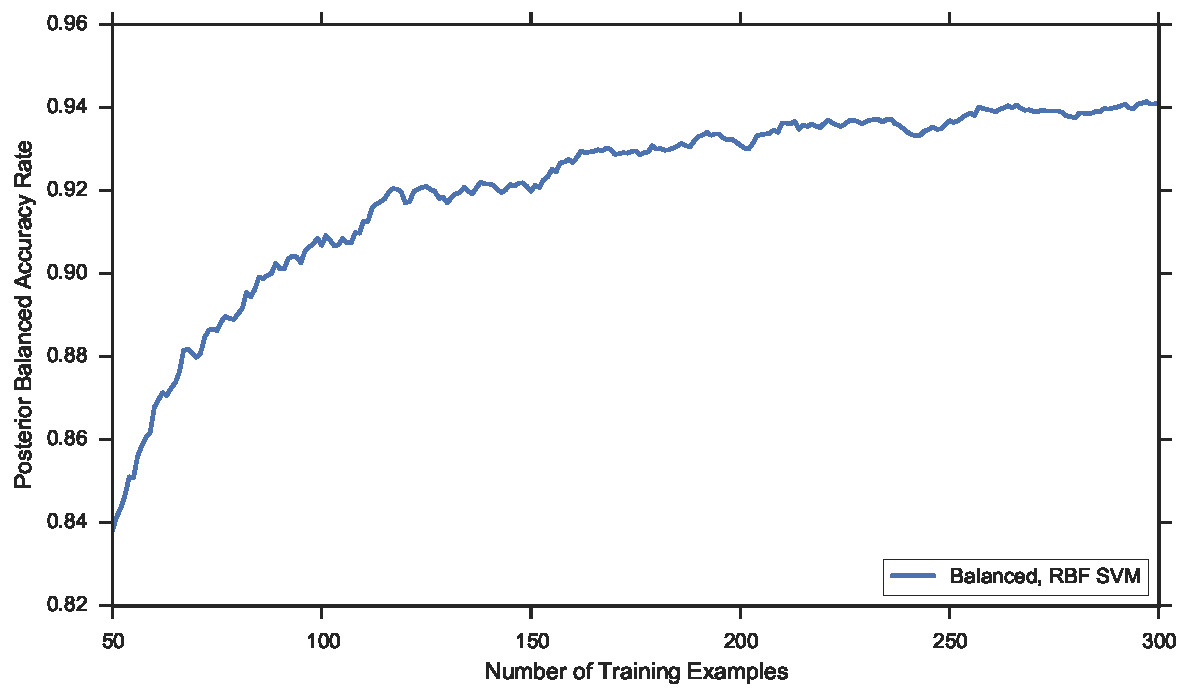
\includegraphics[width=\textwidth]{figures/5_thompson/vstatlas_br_thompson}
	\caption[Learning with Thompson sampling (VST ATLAS, balanced, SVM)]{
		Learning with Thompson sampling (VST ATLAS, balanced, SVM)}
	\label{fig:vstatlas_br_thompson}
\end{figure}

\begin{figure}[p]
	\centering
	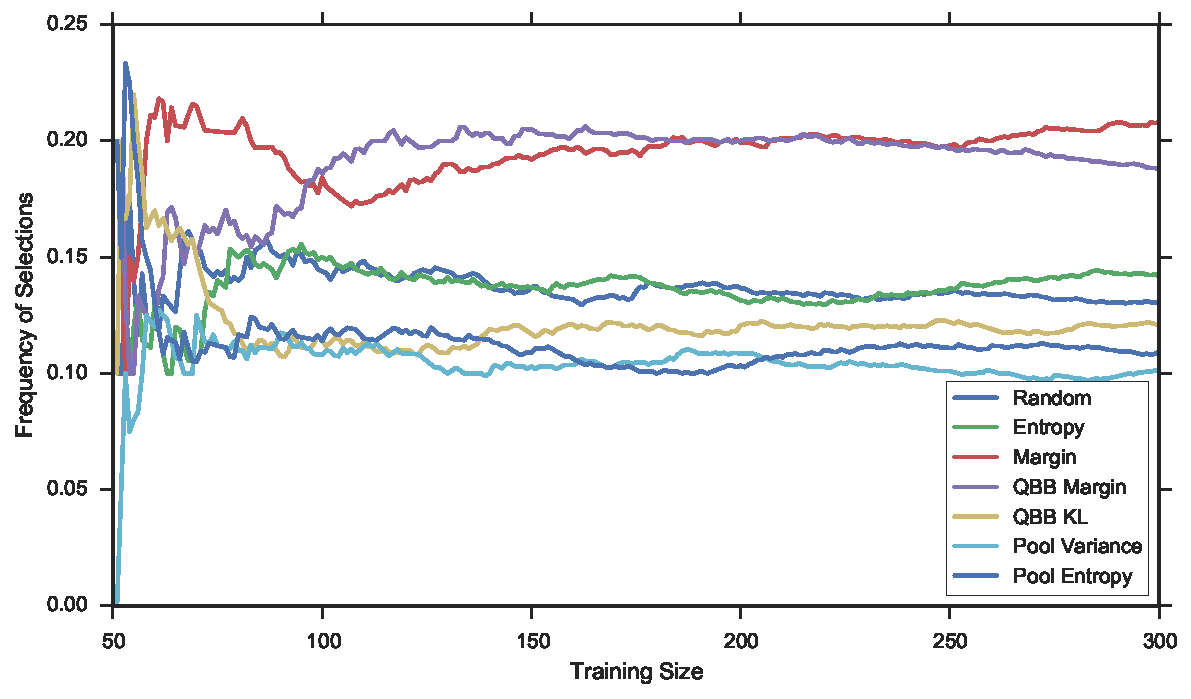
\includegraphics[width=\textwidth]{figures/5_thompson/vstatlas_br_frequencies}
	\caption[Heuristic selection frequency (VST ATLAS, balanced, SVM)]{
		Heuristic selection frequency (VST ATLAS, balanced, SVM)}
	\label{fig:vstatlas_br_frequencies}
\end{figure}

\begin{figure}[p]
	\centering
	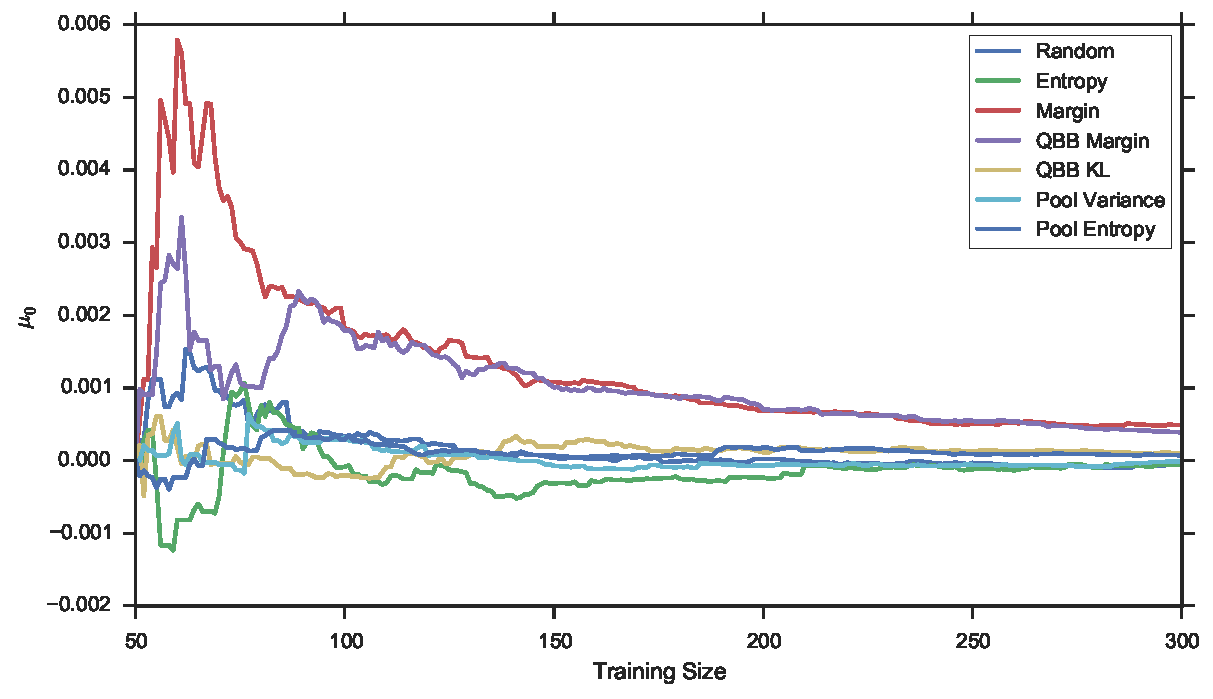
\includegraphics[width=\textwidth]{figures/5_thompson/vstatlas_br_mus}
	\caption[Mean of the reward (VST ATLAS, balanced, SVM)]{
		Mean of the reward (VST ATLAS, balanced, SVM)}
\end{figure}

%--------------------------------------------------------------------------------------------------
\begin{figure}[p]
	\centering
	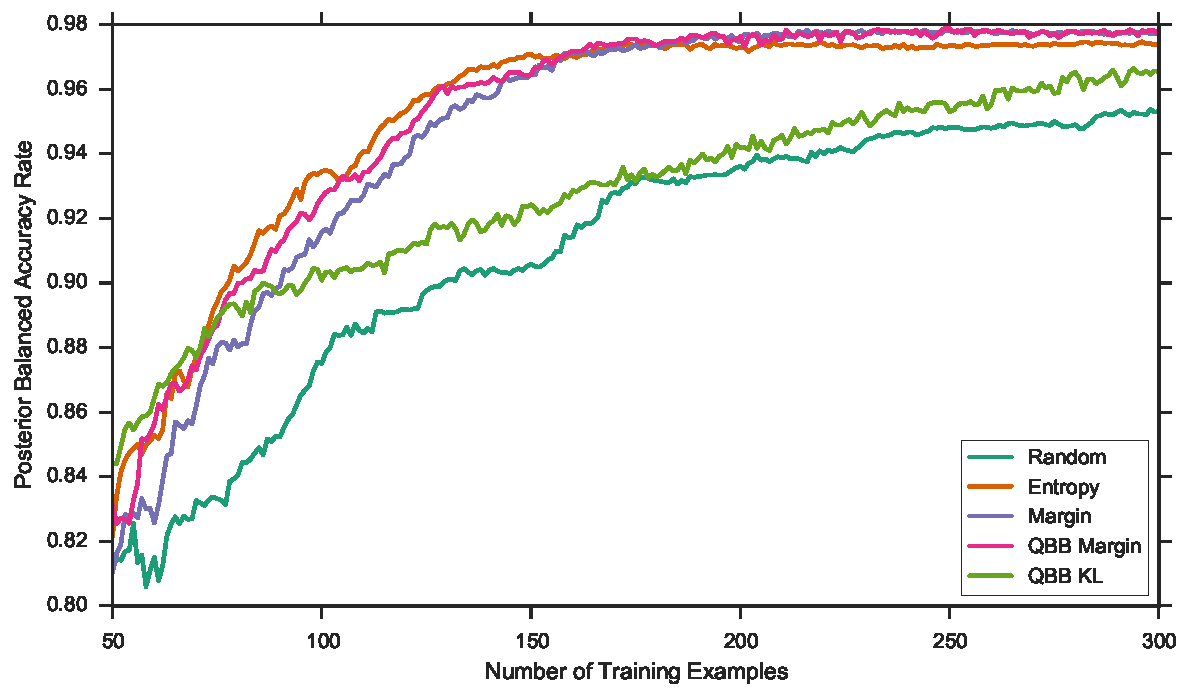
\includegraphics[width=\textwidth]{figures/5_active/vstatlas_ul_individuals}
	\caption[Learning with individual heuristics (VST ATLAS, unbalanced, logistic)]{
		Learning with individual heuristics (VST ATLAS, balanced, logistic)}
	\label{fig:vstatlas_ul_individuals}
\end{figure}

\begin{figure}[p]
	\centering
	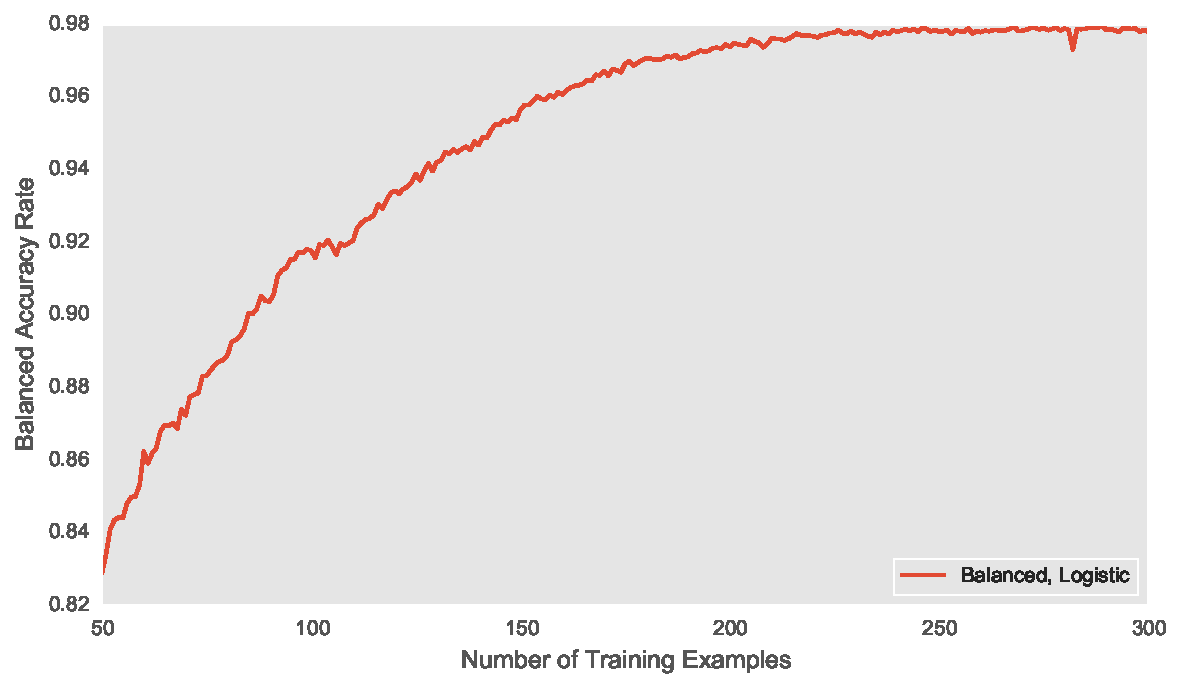
\includegraphics[width=\textwidth]{figures/5_thompson/vstatlas_ul_thompson}
	\caption[Learning with Thompson sampling (VST ATLAS, unbalanced, logistic)]{
		Learning with Thompson sampling (VST ATLAS, balanced, logistic)}
	\label{fig:vstatlas_ul_thompson}
\end{figure}

\begin{figure}[p]
	\centering
	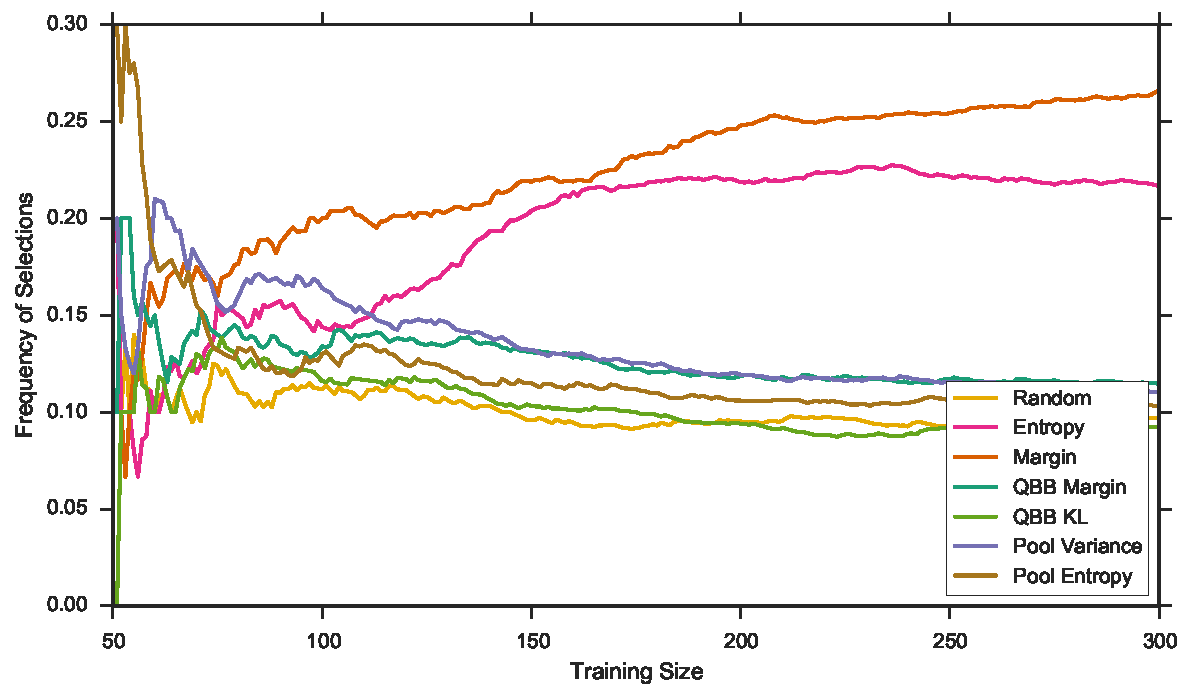
\includegraphics[width=\textwidth]{figures/5_thompson/vstatlas_ul_frequencies}
	\caption[Heuristic selection frequency (VST ATLAS, unbalanced, logistic)]{
		Heuristic selection frequency (VST ATLAS, balanced, logistic)}
	\label{fig:vstatlas_ul_frequencies}
\end{figure}

\begin{figure}[p]
	\centering
	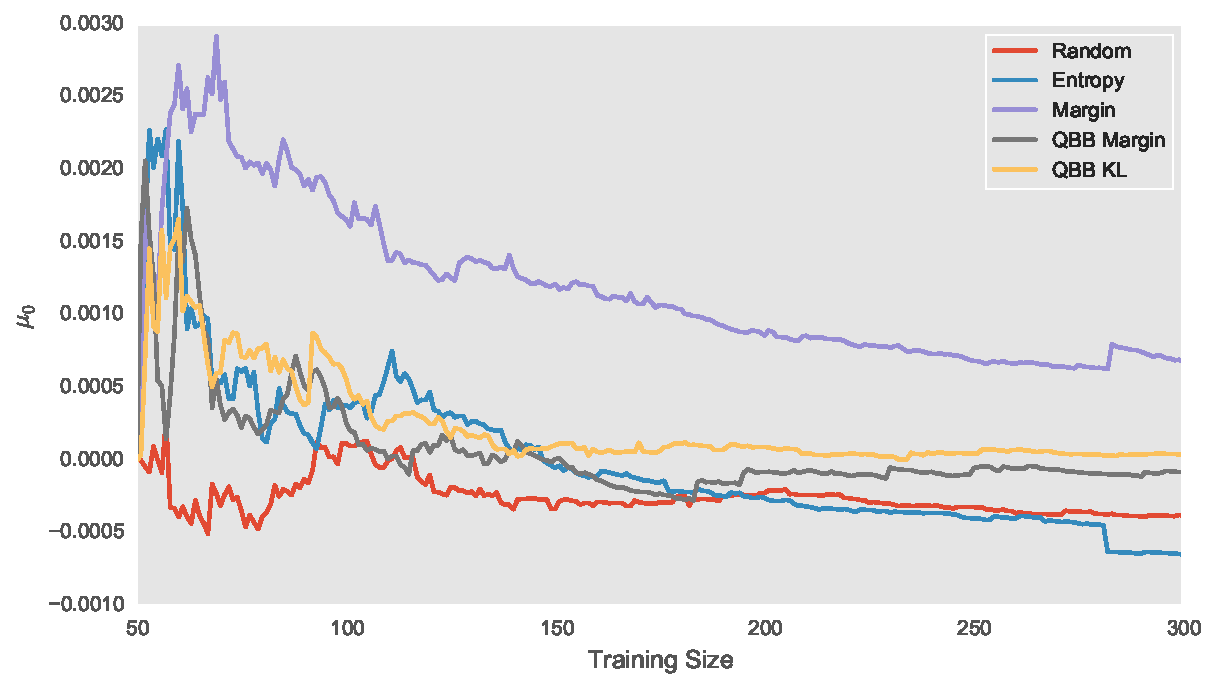
\includegraphics[width=\textwidth]{figures/5_thompson/vstatlas_ul_mus}
	\caption[Mean of the reward (VST ATLAS, unbalanced, logistic)]{
		Mean of the reward (VST ATLAS, balanced, logistic)}
\end{figure}

%--------------------------------------------------------------------------------------------------
\begin{figure}[p]
	\centering
	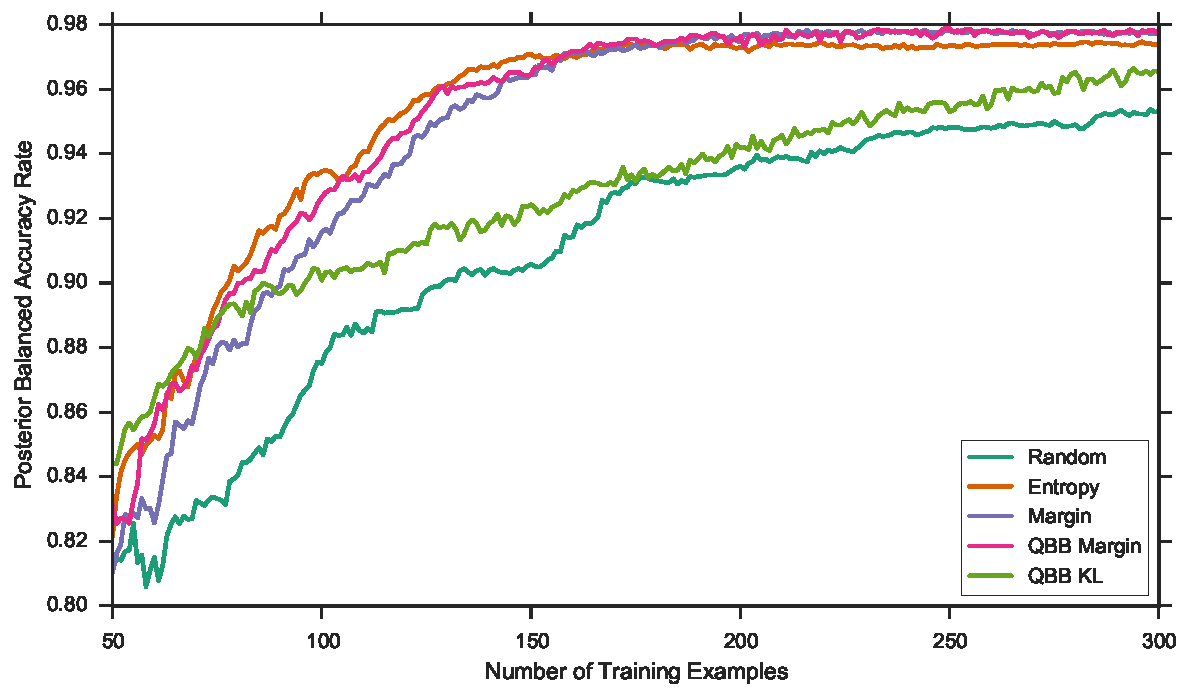
\includegraphics[width=\textwidth]{figures/5_active/vstatlas_ur_individuals}
	\caption[Learning with individual heuristics (VST ATLAS, unbalanced, SVM)]{
		Learning with individual heuristics (VST ATLAS, balanced, SVM)}
	\label{fig:vstatlas_ur_individuals}
\end{figure}

\begin{figure}[p]
	\centering
	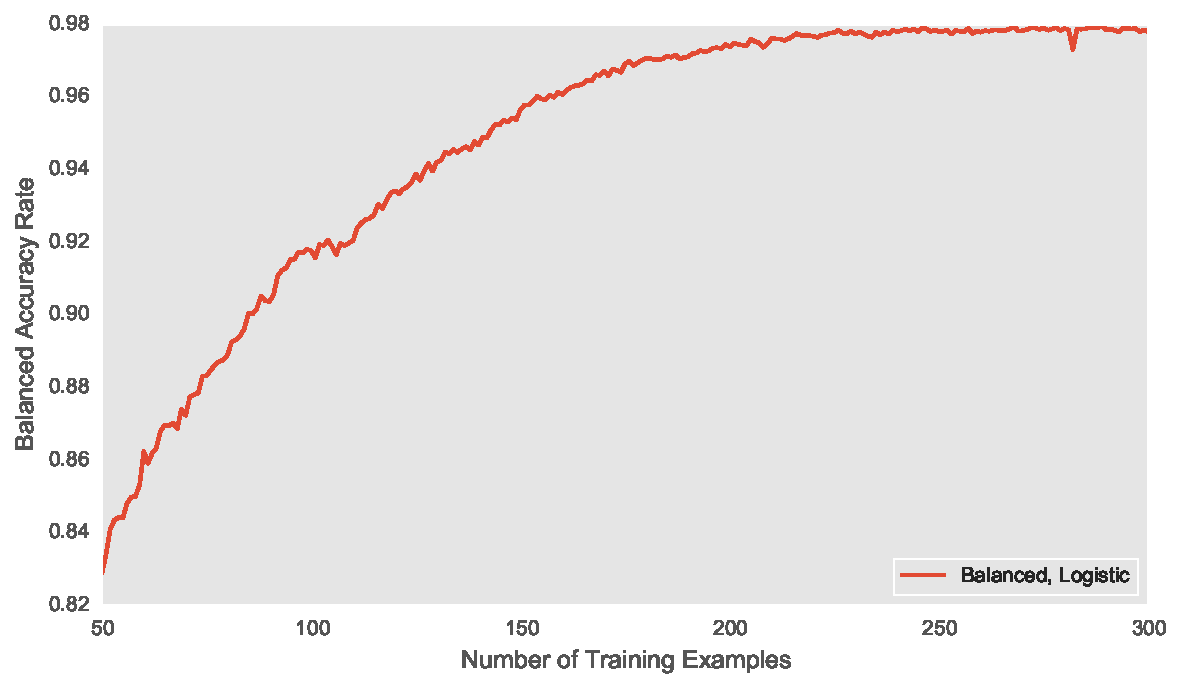
\includegraphics[width=\textwidth]{figures/5_thompson/vstatlas_ur_thompson}
	\caption[Learning with Thompson sampling (VST ATLAS, unbalanced, SVM)]{
		Learning with Thompson sampling (VST ATLAS, balanced, SVM)}
	\label{fig:vstatlas_ur_thompson}
\end{figure}

\begin{figure}[p]
	\centering
	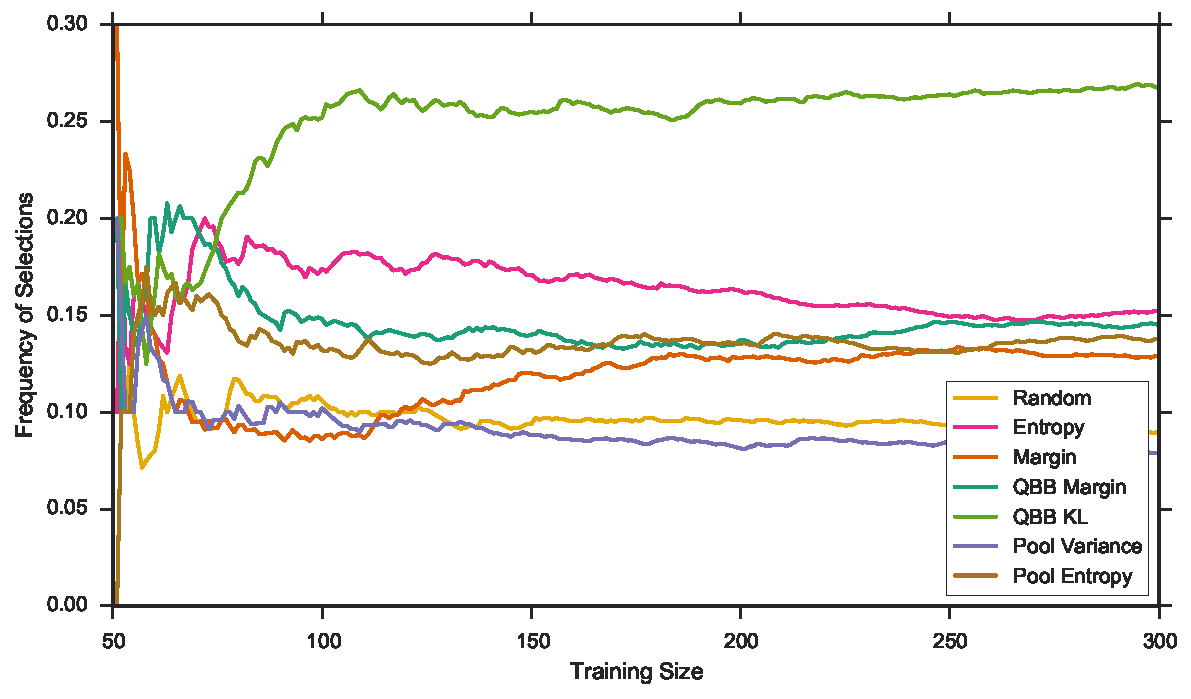
\includegraphics[width=\textwidth]{figures/5_thompson/vstatlas_ur_frequencies}
	\caption[Heuristic selection frequency (VST ATLAS, unbalanced, SVM)]{
		Heuristic selection frequency (VST ATLAS, balanced, SVM)}
	\label{fig:vstatlas_ur_frequencies}
\end{figure}

\begin{figure}[p]
	\centering
	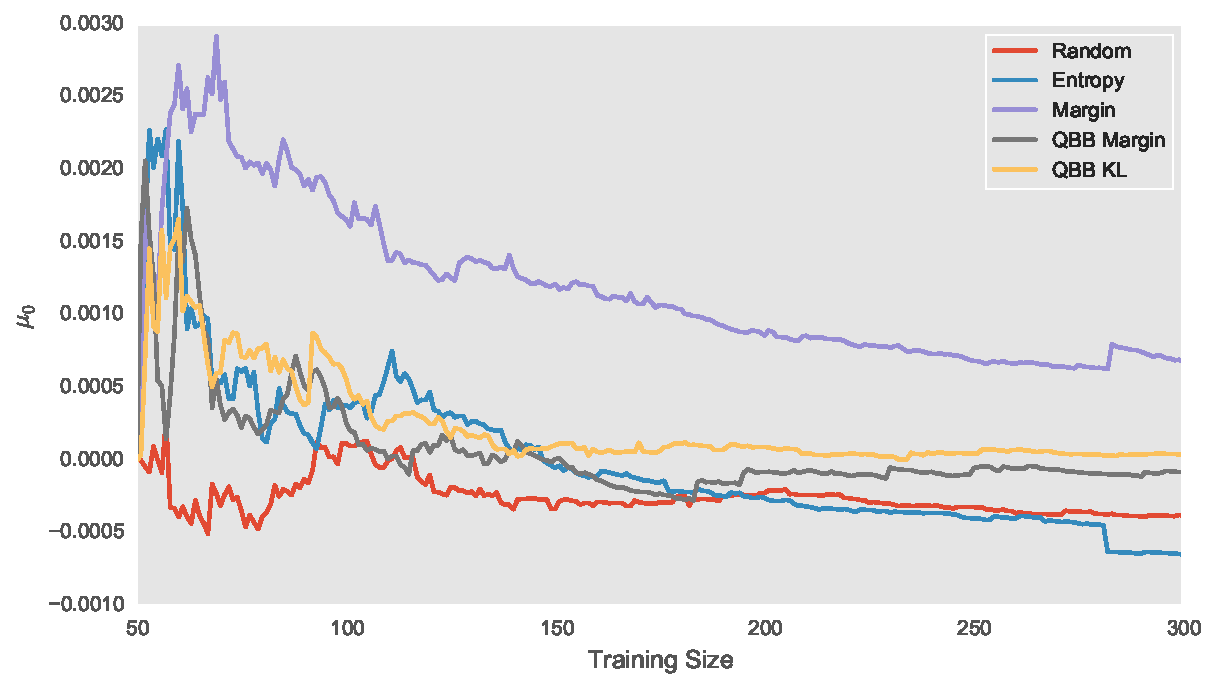
\includegraphics[width=\textwidth]{figures/5_thompson/vstatlas_ur_mus}
	\caption[Mean of the reward (VST ATLAS, unbalanced, SVM)]{
		Mean of the reward (VST ATLAS, balanced, SVM)}
\end{figure}


%%% Local Variables: 
%%% mode: latex
%%% TeX-master: "thesis"
%%% End: 
